\documentclass[11pt,a4paper]{article}
\usepackage[T1]{fontenc}
\usepackage[utf8]{inputenc}
\usepackage{lmodern}
\usepackage[margin=26mm]{geometry}
\usepackage{amsmath,amssymb,amsthm,mathtools}
\usepackage{graphicx,booktabs,array}
\usepackage{microtype}
\usepackage{xcolor}
\definecolor{plum}{HTML}{703D62}
\usepackage[colorlinks=true,linkcolor=plum,citecolor=plum,urlcolor=plum]{hyperref}
\usepackage{enumitem}
\setlist{topsep=4pt,itemsep=4pt,parsep=0pt}
\setlength{\emergencystretch}{2em}
\allowdisplaybreaks[1]
\newtheorem{theorem}{Theorem}[section]
\newtheorem{lemma}[theorem]{Lemma}
\newtheorem{proposition}[theorem]{Proposition}
\newtheorem{corollary}[theorem]{Corollary}
\theoremstyle{definition}
\newtheorem{definition}[theorem]{Definition}
\theoremstyle{remark}
\newtheorem{remark}[theorem]{Remark}
\hypersetup{pdftitle={Reconstruction and continuation in network SIS epidemics},pdfsubject={Version 1.0.0-candidate, DOI 10.5281/zenodo.23524675},pdfauthor={Anonymous}}
\title{Reconstruction and continuation in network SIS epidemics\\[5pt]\large Fixed-dimensional bounds, exponential instability\\and a dimension-free H\"older estimate}
\author{Anonymous}
\date{21 October 2026\\[4pt]\small Version 1.0.0-candidate \quad DOI: \href{https://doi.org/10.5281/zenodo.23524675}{10.5281/zenodo.23524675}\\\small Code and evidence: \url{https://github.com/ipitchford/sis-reconstruction-continuation}}
\begin{document}
\maketitle
\begin{abstract}
Can a network epidemic model fit an observed outbreak accurately and still give an unstable continuation beyond the observation interval? Keliger and Horváth posed a two-part conjecture for the deterministic susceptible--infected--susceptible model: the constant comparing an observable fitting residual on two time intervals should remain bounded first over a fixed-dimensional parameter class, and then over all network sizes. We prove the first assertion and disprove the second. The positive result applies classical polynomial-ideal closure to obtain a scalar differential equation of uniformly bounded order and coefficients at each fixed dimension. The negative result uses complete weighted networks with equal population weights, identical initial infection fractions, and distinct bounded recovery rates. Every example is exactly reconstructible, yet its optimal continuation constant grows at least exponentially with the number of communities. We replace the failed dimension-free linear estimate with an explicit dimension-free Hölder estimate. The same argument gives a direct Hölder bound from past trajectory error to future trajectory error, without differentiating the observations. A corollary converts finitely sampled community-resolved trajectories, with explicit mesh and measurement-error terms, into the same continuation control. We also give nonstationary counterexamples to the proposed block-regularity characterisation of reconstruction, explain their relation to an earlier complete-network solution, and classify all positive invariant rays. The estimates concern this deterministic model and specified error norms. We make no claim that the Hölder exponent is optimal or that its conservative numerical value is useful for forecasting.
\end{abstract}

\section{The question and the result}
\label{sec:introduction}

An epidemic curve records how infection changes over time. A contact matrix records who can infect whom. Different contact matrices can produce the same curve, so recovering a contact matrix and predicting the continuation of a curve are different mathematical tasks. Keliger and Horváth made this distinction precise for a deterministic network epidemic model \cite{KH2026}. They proved a qualitative continuity result for prediction and asked whether a uniform linear error bound also holds.

Here the observation is the full community-resolved vector $z(t)$ over a
continuous interval, not only total prevalence. A sampled-observation
corollary is derived later from the continuous theorem.

This paper resolves the two assertions in their Conjecture 3.11. At every fixed network size, a finite uniform linear bound exists. Across network sizes, no such bound exists, even when every network in the counterexample can be reconstructed uniquely from its exact trajectory. We then prove an explicit Hölder replacement whose constants do not depend on network size. A Hölder estimate allows a small error to be raised to a power below one; it is therefore weaker than a linear estimate near zero, but it still ensures that sufficiently accurate observations give an accurate continuation.

The distinction between exact recovery and stability is essential here. Our negative examples have no exactly invisible direction. They have directions which are extremely difficult to detect during the observation interval and become relatively more visible later. The proof constructs these directions explicitly using the binomial theorem.

\subsection{Model, parameters and observations}

There are $n$ communities. The number $z_i(t)\in[0,1]$ is the infected fraction in community $i$ at time $t$. The population weights satisfy
\[
 \pi_i\geq0,\qquad \sum_{i=1}^n\pi_i=1,
 \qquad \Pi=\operatorname{diag}(\pi_1,\ldots,\pi_n).
\]
The symmetric matrix $W=(w_{ij})$ contains contact weights, including the within-community weights $w_{ii}$. The recovery rates are $\gamma_i\geq0$. The susceptible--infected--susceptible (SIS) equation is
\begin{equation}
 \dot z_i=(1-z_i)(W\Pi z)_i-\gamma_i z_i,
 \qquad i=1,\ldots,n.
 \label{eq:sis}
\end{equation}
All rates and times below use one common time unit. No empirical calibration of that unit is assumed.

For $0<m\leq1/2$ and $M>0$, write $\mathcal P_{m,M}^{(n)}$ for the parameter class used in \cite{KH2026}: every entry of $W$ lies in $[m,M]$, every recovery rate lies in $[0,M]$, and every initial infected fraction lies in $[m,1-m]$. Population weights may vanish for the prediction question. They must be positive for the reconstruction question. When we allow the endpoints $m=0$, the corresponding bounds are $0\leq w_{ij},\gamma_i\leq M$ and $z_i(0)\in[0,1]$.

The cube $[0,1]^n$ is forward invariant. At $z_i=0$ the right side of \eqref{eq:sis} is nonnegative; at $z_i=1$ it is nonpositive. The polynomial vector field therefore has a unique solution for all real $t\geq0$. If $z_i(0)<1$, then $z_i(t)<1$ at every finite time: for $s_i=1-z_i$,
\[
 \dot s_i\geq-Ms_i,\qquad s_i(t)\geq s_i(0)e^{-Mt}>0.
\]

Write $p=(W,\pi,\gamma,z(0))$ for a complete parameter choice. Fix
observation and continuation horizons
\[
 0<T_0<T<\infty.
\]
The trajectory Gram matrix and its associated seminorm are
\begin{equation}
 G_p(S)=\int_0^S z(t)z(t)^T\,dt,
 \qquad
 \|v\|_{G_p(S)}^2=\int_0^S(v^Tz(t))^2\,dt.
 \label{eq:gram}
\end{equation}
We use the \emph{least} admissible continuation constant,
\begin{equation}
 \Lambda(p;T_0,T)=
 \sup_{v:\,\|v\|_{G_p(T_0)}>0}
 \frac{\|v\|_{G_p(T)}}{\|v\|_{G_p(T_0)}}.
 \label{eq:lambda}
\end{equation}
For the zero trajectory we set this constant to one. Specifying the least constant removes an otherwise avoidable ambiguity: an arbitrarily enlarged admissible constant says nothing about uniform boundedness.

For a candidate matrix $\widehat W$, define the observable residual
\begin{equation}
 g(t)=(W-\widehat W)\Pi z(t),\qquad
 H_{2,S}(\widehat W)=
 \left(\int_0^S\|g(t)\|_{2,\pi}^2\,dt\right)^{1/2},
 \quad
 \|x\|_{2,\pi}^2=\sum_i\pi_i|x_i|^2.
 \label{eq:residual}
\end{equation}
When $z_i(t)<1$ for every coordinate, the residual is observable from an exact
differentiable trajectory and known recovery rates, because
\[
 (W\Pi z(t))_i=
 \frac{\dot z_i(t)+\gamma_i z_i(t)}{1-z_i(t)}.
\]
At a saturated coordinate with $z_i=1$, the residual remains algebraically
defined but this division formula need not be available. It is not the same
quantity as the error between two infected-fraction trajectories.
Section~\ref{sec:holder} also gives a bound directly for that latter quantity.

\subsection{What the proofs establish}

The conclusions are as follows.
\begin{enumerate}
 \item For fixed $n,M,T_0,T$, the constant in \eqref{eq:lambda} is uniformly bounded over the entire parameter class. The proof even permits $m=0$; see Section~\ref{sec:fixed}.
 \item There are exactly reconstructible examples in the fixed class $\mathcal P_{1/4,2}^{(d+1)}$ whose optimal constants $\Lambda_d$ satisfy
 \[
   \liminf_{d\to\infty}\Lambda_d^{1/d}\geq T/T_0>1.
 \]
 Symmetric candidate networks in the same parameter box realise this amplification in the residual \eqref{eq:residual}; see Section~\ref{sec:negative}.
 \item Uniform boundedness of the coefficients still yields a dimension-free Hölder continuation estimate. We give all constants and prove the estimate by an elementary interpolation argument in Section~\ref{sec:holder}.
 \item Nonstationary failure of network reconstruction need not arise from block regularity. Section~\ref{sec:reconstruction} describes the full affine ambiguity space of any given trajectory and gives examples with distinct initial infected fractions.
\end{enumerate}

The tools behind some of these statements have substantial prior history. Novikov and Yakovenko already developed the polynomial-ideal reduction from nonlinear trajectories to scalar linear differential equations \cite[Sections 2.2--2.3]{NY1999}. Prasse, Devriendt and Van Mieghem already obtained the rank-two complete-network solution used in one reconstruction counterexample \cite[Theorem 4]{PDM2021}. Hölder control for bounded analytic continuation is also classical; Trefethen gives a quantitative account of the general principle and continuation along chains of discs \cite{T2020}. Our contribution is the stated resolution of the SIS continuation conjecture, its explicit dimension-free SIS replacement, and the precise reconstruction consequences and examples. We do not claim any of these general methods as new.

\section{A uniform bound at every fixed dimension}
\label{sec:fixed}

Compactness of the parameter box alone does not settle this question. A Gram matrix can acquire a larger kernel at a limiting parameter, and its smallest positive eigenvalue can tend to zero. We must control how the observed functions approach that singular limit. The polynomial structure of \eqref{eq:sis} provides the needed control.

The proof has two steps. First, a scalar function which satisfies a linear differential equation of fixed order with bounded coefficients cannot be arbitrarily small on an initial interval relative to its derivative state. Second, polynomial-ideal closure supplies just such an equation for every output $v^Tz(t)$, uniformly over a fixed-dimensional parameter box.

\begin{lemma}[Observation of a scalar equation]
\label{lem:companion}
Fix $r\geq1$, $B\geq0$ and $0<T_0<T$. There is a finite constant $C=C(r,B,T_0,T)$ such that every solution of
\begin{equation}
 h^{(r)}(t)=\sum_{j=0}^{r-1}b_j(t)h^{(j)}(t),
 \qquad |b_j(t)|\leq B,
 \label{eq:scalar}
\end{equation}
satisfies
\[
 \int_0^T|h(t)|^2\,dt
 \leq C\int_0^{T_0}|h(t)|^2\,dt.
\]
Bounded measurable coefficients are sufficient, with the derivative state interpreted as an absolutely continuous solution of the companion system.
\end{lemma}

\begin{proof}
Put $U=(h,h',\ldots,h^{(r-1)})^T$. The first $r-1$ rows of its companion matrix shift one coordinate to the next; its last row contains the $b_j$. Its norm is bounded by some $K=K(r,B)$, so Gronwall's inequality gives
\begin{equation}
 |U(t)|\leq e^{Kt}|U(0)|.
 \label{eq:state-growth}
\end{equation}
We claim that there is $c=c(r,B,T_0)>0$ such that
\begin{equation}
 \int_0^{T_0}|h(t)|^2\,dt\geq c|U(0)|^2.
 \label{eq:observation-lower}
\end{equation}
Suppose otherwise. Rescale a contradicting sequence so that $|U_k(0)|=1$ while the output integrals tend to zero. Equation~\eqref{eq:state-growth} bounds $U_k$ uniformly. The companion equation also bounds $U_k'$ uniformly. Arzelà--Ascoli therefore gives a uniformly convergent subsequence on $[0,T_0]$, with limit $U_*$. Its first coordinate is identically zero, because its squared integral is zero.

For every $j=0,\ldots,r-2$, the identities
\[
 (U_k)_j(t)=(U_k)_j(0)+\int_0^t(U_k)_{j+1}(s)\,ds
\]
pass to the uniform limit. The derivative of the first coordinate of $U_*$ is consequently its second coordinate. Since the first coordinate is zero, the second is zero. Repeating the argument shows that every coordinate is zero. This contradicts $|U_*(0)|=1$ and proves \eqref{eq:observation-lower}. Notice that the argument does not require convergence of the final-row coefficients.

Finally,
\[
 \int_0^T|h(t)|^2\,dt
 \leq Te^{2KT}|U(0)|^2
 \leq \frac{Te^{2KT}}c\int_0^{T_0}|h(t)|^2\,dt.
\]
\end{proof}

\begin{theorem}[Fixed-dimensional continuation]
\label{thm:fixed}
For every fixed $n,M,T_0,T$ with $0<T_0<T$, there is a finite constant $C_n=C_n(M,T_0,T)$ such that every solution of \eqref{eq:sis} with
\[
 0\leq w_{ij},\gamma_i\leq M,\qquad
 \pi_i\geq0,\quad\sum_i\pi_i=1,\qquad z(0)\in[0,1]^n
\]
satisfies
\begin{equation}
 \int_0^T(v^Tz(t))^2\,dt
 \leq C_n\int_0^{T_0}(v^Tz(t))^2\,dt
 \qquad(v\in\mathbb R^n).
 \label{eq:fixed-bound}
\end{equation}
In particular, Conjecture 3.11, equation (14), of \cite{KH2026} holds. Symmetry of $W$ is not needed for this bound.
\end{theorem}

\begin{proof}
We give the polynomial-ideal argument, following the general construction in \cite[Sections 2.2--2.3]{NY1999}. Let $\vartheta$ collect the entries of $W$, $\pi$ and $\gamma$. Treat them as independent indeterminates which remain constant along a trajectory. Also treat the entries of $v$ as constant indeterminates. In the polynomial ring
\[
 \mathcal R=\mathbb R[z,\vartheta,v]
\]
define
\[
 p_0=v^Tz,\qquad
 p_{j+1}=\mathcal L_Fp_j
 :=\sum_{i=1}^nF_i(z;\vartheta)\frac{\partial p_j}{\partial z_i},
\]
where $F$ is the right side of \eqref{eq:sis}. The operator $\mathcal L_F$ simply differentiates a polynomial along solutions of the differential equation.

The ideals
\[
 (p_0)\subseteq(p_0,p_1)\subseteq\cdots
\]
form an increasing sequence in a polynomial ring with finitely many variables. Hilbert's basis theorem says that this sequence eventually stabilises. Thus, for some finite $r$ and some polynomials $a_0,\ldots,a_{r-1}$ in $\mathcal R$,
\begin{equation}
 p_r=\sum_{j=0}^{r-1}a_j(z,\vartheta,v)p_j.
 \label{eq:ideal-closure}
\end{equation}
This is a polynomial identity in all the parameters. In particular, the argument does not divide by a Gram determinant or by any quantity that might vanish at a singular parameter.

By homogeneity of \eqref{eq:fixed-bound}, it is enough to consider $|v|=1$. The state remains in $[0,1]^n$, the parameters remain in their bounded boxes and simplex, and $v$ lies on a compact sphere. Hence all the polynomials $a_j$ in \eqref{eq:ideal-closure} have one common finite bound $B$ on this set.

Along a solution,
\[
 p_j(z(t),\vartheta,v)=\frac{d^j}{dt^j}(v^Tz(t)).
\]
Consequently \eqref{eq:ideal-closure} is a scalar equation of the form \eqref{eq:scalar}, with one fixed order $r$ and one coefficient bound $B$ for the entire parameter class. Lemma~\ref{lem:companion} proves \eqref{eq:fixed-bound}. The case $v=0$ is immediate.
\end{proof}

\begin{corollary}[Residual bound at fixed dimension]
\label{cor:fixed-residual}
Under the assumptions of Theorem~\ref{thm:fixed}, every candidate matrix $\widehat W$ satisfies
\[
 H_{2,T}(\widehat W)\leq\sqrt{C_n}\,H_{2,T_0}(\widehat W).
\]
\end{corollary}

\begin{proof}
Each coordinate of $(W-\widehat W)\Pi z(t)$ is a linear output of the trajectory. Apply \eqref{eq:fixed-bound} to each row, multiply by $\pi_i$, and add.
\end{proof}

Theorem~\ref{thm:fixed} proves existence of a uniform constant, not a useful numerical value for it. Exact ideal membership and coefficient bounds could in principle produce a computable constant. We have not carried out that computation. Polynomial-ring methods also occur in finite tests for nonlinear observability \cite{KO2013}; our use here is the particular interval comparison proved above.

\section{Exponential failure across network sizes}
\label{sec:negative}

We now keep all coefficients in one fixed box while allowing the number of communities to grow. The contact network is as simple as possible: all its weights are one. Only the recovery rates vary. This variation produces many distinct time profiles. A binomial combination cancels their first responses and leaves a signal which is much smaller early than later.

\subsection{An exactly reconstructible family}

For an integer $d\geq1$, index the $n=d+1$ communities by $i=0,\ldots,d$ and choose
\begin{equation}
 W=\mathbf1\mathbf1^T,\qquad
 \pi_i=\frac1{d+1},\qquad
 z_i(0)=\frac12,\qquad
 \gamma_i=\frac{i}{d}.
 \label{eq:negative-family}
\end{equation}
These parameters belong to $\mathcal P_{1/4,2}^{(d+1)}$ for every $d$. Let
\[
 a(t)=\frac1{d+1}\sum_{i=0}^dz_i(t),\qquad
 A(t)=\int_0^ta(s)\,ds.
\]
The common infection force is $a(t)$, and each coordinate satisfies
\[
 \dot z_i+(a(t)+\gamma_i)z_i=a(t).
\]
Variation of constants gives
\begin{equation}
 z_i(t)=e^{-A(t)}\left[
  \frac12e^{-\gamma_it}
  +\int_0^ta(s)e^{A(s)}e^{-\gamma_i(t-s)}\,ds
 \right].
 \label{eq:variation}
\end{equation}
The function $a$ is determined by the coupled model. We do not replace it by an externally imposed forcing. Its bounds $0\leq a\leq1$ will be enough.

\begin{proposition}[Exact reconstruction in the negative family]
\label{prop:reconstructible}
For every $d\geq1$ and $S>0$, the matrix $G_p(S)$ for \eqref{eq:negative-family} is positive definite. Thus its contact matrix is reconstructible from its exact trajectory and the other known parameters.
\end{proposition}

\begin{proof}
Suppose $v^Tz(t)=0$ on $[0,S]$. Set
\[
 q_v(t)=\sum_{i=0}^dv_i e^{-\gamma_it}.
\]
Taking the same linear combination in \eqref{eq:variation} gives
\[
 \frac12q_v(t)+\int_0^ta(s)e^{A(s)}q_v(t-s)\,ds=0.
\]
The kernel $a(s)e^{A(s)}$ is bounded on $[0,S]$. For a finite constant $K_S$ this implies
\[
 |q_v(t)|\leq K_S\int_0^t|q_v(u)|\,du.
\]
Gronwall's inequality gives $q_v=0$. Differentiating at zero for $k=0,\ldots,d$ yields
\[
 \sum_{i=0}^dv_i(-\gamma_i)^k=0.
\]
This Vandermonde system is invertible because the recovery rates are distinct. Hence $v=0$. If $v^TG_p(S)v=0$, continuity first gives $v^Tz=0$ on the interval, so the same argument proves positive definiteness. Reconstruction then follows from the Gram criterion in \cite[Theorem 3.1]{KH2026}, or directly by subtracting the two network equations.
\end{proof}

\subsection{The cancelling output}

Choose
\begin{equation}
 v_i=(-1)^i\binom di,\qquad
 h_d(t)=\sum_{i=0}^dv_i z_i(t),\qquad
 f_d(t)=(1-e^{-t/d})^d.
 \label{eq:binomial}
\end{equation}
The binomial theorem gives
\[
 \sum_{i=0}^dv_i e^{-\gamma_it}=f_d(t).
\]
Therefore \eqref{eq:variation} becomes the exact identity
\begin{equation}
 h_d(t)=e^{-A(t)}\left[
  \frac12f_d(t)+\int_0^ta(s)e^{A(s)}f_d(t-s)\,ds
 \right].
 \label{eq:positive-convolution}
\end{equation}
An alternating sum of coordinates has become a sum of nonnegative terms. This identity supplies both the proof and a stable way to evaluate the small output numerically.

\begin{lemma}[Two bounds for the cancelling output]
\label{lem:output-bounds}
For every $t\geq0$,
\begin{equation}
 \frac12e^{-t}f_d(t)\leq h_d(t)\leq f_d(t).
 \label{eq:output-bounds}
\end{equation}
In particular, $h_d(t)>0$ when $t>0$.
\end{lemma}

\begin{proof}
For the lower bound, discard the nonnegative integral in \eqref{eq:positive-convolution} and use $A(t)\leq t$. For the upper bound, $f_d$ is increasing, so
\begin{align*}
 h_d(t)
 &\leq f_d(t)\left[
  \frac12e^{-A(t)}+
  \int_0^ta(s)e^{A(s)-A(t)}\,ds\right]\\
 &=f_d(t)\left[\frac12e^{-A(t)}+1-e^{-A(t)}\right]
 \leq f_d(t).
\end{align*}
\end{proof}

\begin{theorem}[Dimension-free linear continuation fails]
\label{thm:exponential}
Let $\Lambda_d=\Lambda(p_d;T_0,T)$ for the family \eqref{eq:negative-family}. For every $s$ with $T_0<s<T$,
\begin{equation}
 \Lambda_d\geq
 \frac12e^{-T}\sqrt{\frac{T-s}{T_0}}
 \left(\frac{1-e^{-s/d}}{1-e^{-T_0/d}}\right)^d
 \geq
 \frac12e^{-T-s}\sqrt{\frac{T-s}{T_0}}
 \left(\frac{s}{T_0}\right)^d.
 \label{eq:exponential-bound}
\end{equation}
Consequently,
\begin{equation}
 \liminf_{d\to\infty}\Lambda_d^{1/d}\geq\frac{T}{T_0}>1.
 \label{eq:exponential-rate}
\end{equation}
For the displayed binomial output itself, the exponential rate is exact:
\begin{equation}
 \lim_{d\to\infty}
 \left(\frac{\|h_d\|_{L^2(0,T)}}{\|h_d\|_{L^2(0,T_0)}}\right)^{1/d}
 =\frac{T}{T_0}.
 \label{eq:direction-exact-rate}
\end{equation}
This disproves Conjecture 3.11, equation (15), of \cite{KH2026}.
\end{theorem}

\begin{proof}
Use the vector in \eqref{eq:binomial} in the supremum \eqref{eq:lambda}. Lemma~\ref{lem:output-bounds} gives
\[
 \|h_d\|_{L^2(0,T_0)}\leq\sqrt{T_0}f_d(T_0),\qquad
 \|h_d\|_{L^2(0,T)}\geq
 \frac12e^{-T}\sqrt{T-s}\,f_d(s).
\]
This proves the first inequality in \eqref{eq:exponential-bound}. The elementary bounds
\[
 xe^{-x}\leq1-e^{-x}\leq x\qquad(x\geq0)
\]
give
\[
 \left(\frac{1-e^{-s/d}}{1-e^{-T_0/d}}\right)^d
 \geq e^{-s}\left(\frac{s}{T_0}\right)^d,
\]
which proves the second inequality. Taking $d$th roots gives a lower limit of at least $s/T_0$ for every fixed $s<T$. Let $s$ increase to $T$ to obtain \eqref{eq:exponential-rate}.

To prove \eqref{eq:direction-exact-rate}, the same lower bound applies to the displayed output ratio. In the other direction, for $0<u<T_0$, Lemma~\ref{lem:output-bounds} gives
\[
 \frac{\|h_d\|_{L^2(0,T)}}{\|h_d\|_{L^2(0,T_0)}}
 \leq2e^{T_0}\sqrt{\frac{T}{T_0-u}}\,\frac{f_d(T)}{f_d(u)}.
\]
The $d$th root of the last fraction tends to $T/u$. Letting $u$ increase to $T_0$ proves the matching upper limit. This last assertion concerns the specified direction; no matching upper bound for the optimal $\Lambda_d$ is claimed.
\end{proof}

\begin{corollary}[The residual has the same obstruction]
\label{cor:negative-residual}
Let $v$ be as in \eqref{eq:binomial}, and choose
\[
 0<\varepsilon_d\leq
 \frac{1}{2\max_i\binom di^2},\qquad
 \widehat W_d=W+\varepsilon_d vv^T.
\]
Both networks are symmetric and all entries of $\widehat W_d$ lie in $[1/2,3/2]$. Moreover,
\[
 \frac{H_{2,T}(\widehat W_d)}{H_{2,T_0}(\widehat W_d)}
 =\frac{\|h_d\|_{L^2(0,T)}}{\|h_d\|_{L^2(0,T_0)}},
\]
so the lower bounds in \eqref{eq:exponential-bound} apply to admissible fitting residuals as well.
\end{corollary}

\begin{proof}
The entry bound follows from $|v_iv_j|\leq\max_kv_k^2$. Since $\Pi=I/(d+1)$,
\[
 (\widehat W_d-W)\Pi z(t)
 =\frac{\varepsilon_d}{d+1}v\,h_d(t).
\]
The fixed positive vector-norm factor cancels in the ratio.
\end{proof}

The large ratio does not imply a large absolute forecasting error. The binomial coefficients grow, while $h_d(t)$ is extremely small for fixed $t$ and large $d$. The chosen perturbation also shrinks to keep the candidate matrix within its coefficient box. The theorem rules out one uniform \emph{relative linear} bound; it does not contradict qualitative uniform continuity or the Hölder estimate proved next. It also does not, by itself, disprove a linear bound between two actual trajectory errors in a different norm. Figure~\ref{fig:growth} compares the specified direction with the rigorous lower bound; its solid curve is not the optimal $\Lambda_d$.

\begin{figure}[tb]
 \centering
 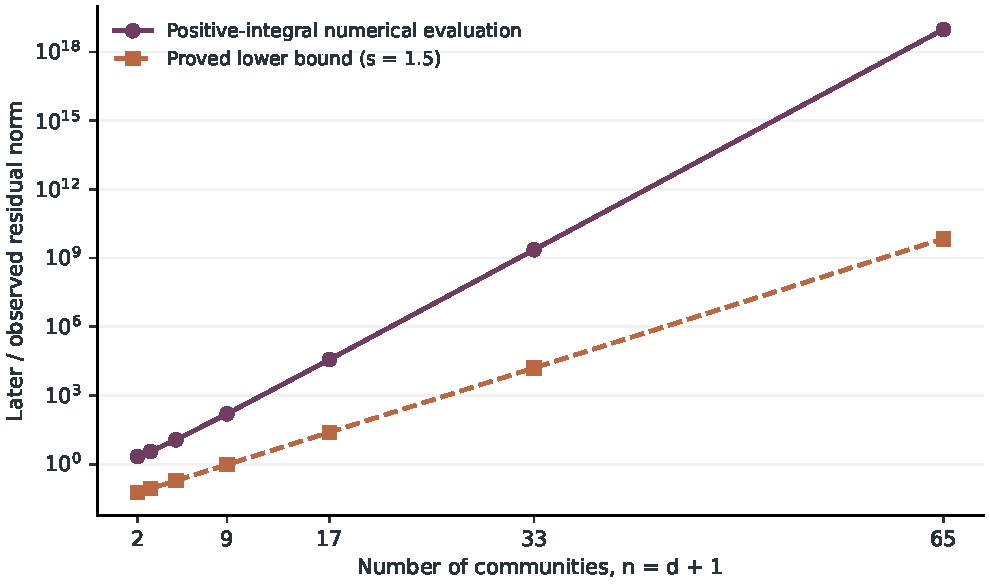
\includegraphics[width=.85\linewidth]{figures/sis_growth.pdf}
 \caption{Continuation amplification for the explicit binomial direction, with $T_0=1$ and $T=2$. The solid curve is a numerical evaluation of the positive integral \eqref{eq:positive-convolution}; it reaches approximately $9.61\times10^{18}$ at $n=65$. The dashed curve is the rigorous first lower bound in \eqref{eq:exponential-bound}, evaluated at $s=1.5$, which exceeds $6.94\times10^9$ there. The plotted quantity is the residual-norm ratio in Corollary~\ref{cor:negative-residual}. Numerical values illustrate the theorem and are not used in its proof.}
 \label{fig:growth}
\end{figure}

\section{An explicit dimension-free Hölder replacement}
\label{sec:holder}

The negative result leaves a useful positive question: how does a small observation error control continuation when the number of communities is unrestricted? Bounded contact and recovery rates give a common complex-time neighbourhood on which all trajectories are analytic and bounded. Polynomial interpolation then transfers a small bound a short distance along the real axis. Repeating that transfer gives an explicit Hölder estimate.

The bounded-analytic-continuation principle and its Hölder dependence are classical; see \cite[Theorem 5.2 and Section 7]{T2020}. The work here is to establish a common analytic bound for the SIS model independently of its dimension, and to give explicit constants for the required interval norms. The constants below are deliberately conservative. Their role is to prove a uniform rate, not to prescribe the measurement precision of a real forecasting system.

For $M>0$, define
\begin{align}
 r&=\min\left\{T_0,\frac1{120M}\right\},
 &K&=\left\lceil\frac{T-T_0}{r}\right\rceil,
 &\theta&=\frac{\log2}{\log(8e)},\label{eq:holder-constants-a}\\
 C_0&=2\max\{1,(MT_0)^{1/3}\},
 &\beta&=\frac23\theta^K,
 &C_*&=\left(\frac94\right)^{(1-\theta^K)/(1-\theta)}C_0^{\theta^K}.
 \label{eq:holder-constants-b}
\end{align}

\begin{theorem}[Dimension-free continuation of the residual]
\label{thm:holder-residual}
Suppose $0\leq w_{ij},\widehat w_{ij},\gamma_i\leq M$, $\pi$ is any probability vector, and $z(0)\in[0,1]^n$. Set
\[
 E=H_{2,T_0}(\widehat W),\qquad B=2M.
\]
Then
\begin{equation}
 H_{2,T}(\widehat W)
 \leq B\sqrt T\,C_*
 \left(\frac{E}{B\sqrt{T_0}}\right)^\beta.
 \label{eq:holder-residual}
\end{equation}
The constants depend only on $M,T_0,T$, and do not depend on the dimension, population weights, matrices, recovery rates or initial conditions. Symmetry of the two matrices is unnecessary for this estimate.
\end{theorem}

We prove the theorem through three elementary lemmas. The first supplies a common analytic neighbourhood. The second converts an integral observation error into a uniform error on the observed interval. The third continues that uniform error one short step forward.

\begin{lemma}[A common complex-time disc]
\label{lem:analytic-disc}
At every real centre $c\geq0$, a solution of \eqref{eq:sis} has a holomorphic extension to the complex disc
\[
 |t-c|<\rho,\qquad \rho=\frac1{12M},
\]
on which $\|z(t)\|_\infty\leq2$. On that disc, the residual in \eqref{eq:residual} satisfies $\|g(t)\|_{2,\pi}\leq2M$. On the real axis, $\|g'(t)\|_{2,\pi}\leq2M^2$.
\end{lemma}

\begin{proof}
The real state $z(c)$ lies in $[0,1]^n$. In the complex ball $\|y-z(c)\|_\infty\leq1$, both $\|y\|_\infty$ and $\|\mathbf1-y\|_\infty$ are at most two. The row sums of $W\Pi$ are at most $M$, so
\[
 \|F(y)\|_\infty\leq6M.
\]
The three terms in the derivative
\[
 DF(y)u=-\operatorname{diag}(W\Pi y)u
  +\operatorname{diag}(\mathbf1-y)W\Pi u
  -\operatorname{diag}(\gamma)u
\]
have norms at most $2M$, $2M$ and $M$. Hence $F$ has Lipschitz constant at most $5M$ in that ball. Complex Picard iteration on the disc of radius $\rho$ moves a function by at most $6M\rho=1/2$ and contracts by a factor at most $5M\rho=5/12$. It gives the stated holomorphic solution and bound, independently of $n$.

Since both $W$ and $\widehat W$ have entries in $[0,M]$, every entry of their difference has absolute value at most $M$. Thus
\[
 \|(W-\widehat W)\Pi y\|_\infty\leq M\|y\|_\infty\leq2M.
\]
The weighted Hilbert norm is at most the sup norm. On the real axis the separate infection and recovery terms give $\|z'\|_\infty\leq2M$, so the same matrix bound gives $\|g'\|_{2,\pi}\leq2M^2$.
\end{proof}

\begin{lemma}[From an integral error to a uniform error]
\label{lem:l2-sup}
Let $f$ take values in a Hilbert space, with $\|f\|\leq1$ and Lipschitz constant at most $M$ on $[0,T_0]$. Put
\[
 \epsilon=\frac{\|f\|_{L^2(0,T_0)}}{\sqrt{T_0}}\in[0,1].
\]
Then
\[
 \sup_{0\leq t\leq T_0}\|f(t)\|\leq C_0\epsilon^{2/3}.
\]
\end{lemma}

\begin{proof}
For $0<s\leq T_0$ and a given $t\in[0,T_0]$, choose an interval of length $s$ contained in $[0,T_0]$ and containing $t$. Average the Lipschitz inequality over that interval and apply Cauchy--Schwarz. This gives
\[
 \|f(t)\|\leq\epsilon\sqrt{T_0/s}+Ms.
\]
If $\epsilon<MT_0$, take $s=T_0(\epsilon/(MT_0))^{2/3}$. Both terms then equal $(MT_0)^{1/3}\epsilon^{2/3}$. If $\epsilon\geq MT_0$, take $s=T_0$ and use $\epsilon+MT_0\leq2\epsilon\leq2\epsilon^{2/3}$. The zero case follows by continuity, or directly from continuity of $f$ and its zero integral.
\end{proof}

\begin{lemma}[One continuation step]
\label{lem:one-step}
Let a Hilbert-valued function $f$ be holomorphic and bounded in norm by one on the disc $|t-c|<5r$. If
\[
 \sup_{c-r\leq t\leq c}\|f(t)\|\leq\delta\leq1,
\]
then
\begin{equation}
 \sup_{c\leq t\leq c+r}\|f(t)\|
 \leq\frac94\delta^\theta,
 \qquad \theta=\frac{\log2}{\log(8e)}.
 \label{eq:one-step}
\end{equation}
\end{lemma}

\begin{proof}
For an integer $N\geq1$, interpolate $f$ at the $N+1$ equally spaced nodes
\[
 x_j=c-r+\frac{jr}{N},\qquad j=0,\ldots,N.
\]
For $t\in[c,c+r]$, the absolute sum of the Lagrange factors satisfies
\[
 \sum_{j=0}^N|L_j(t)|
 \leq(2N)^N\sum_{j=0}^N\frac1{j!(N-j)!}
 =\frac{(4N)^N}{N!}\leq(4e)^N.
\]
The interpolation polynomial therefore has norm at most $(4e)^N\delta$ on the new interval.

For the remainder, integrate the Cauchy interpolation formula on $|\zeta-c|=5r$, or first on a smaller circle and pass to the limit. On the larger circle,
\[
 |t-x_j|\leq2r,\qquad |\zeta-x_j|\geq4r,
 \qquad |\zeta-t|\geq4r.
\]
The contour-length factor then gives
\[
 \|f(t)-P_N(t)\|\leq\frac54\,2^{-N-1}.
\]
For $N=0$, use the single node $c$; the same, slightly loose, remainder bound holds. Thus for every $N\geq0$,
\begin{equation}
 \sup_{[c,c+r]}\|f\|
 \leq(4e)^N\delta+\frac54\,2^{-N-1}.
 \label{eq:interpolation-bound}
\end{equation}
The formulas hold componentwise, and their norm estimates are dimension independent. Equivalently, one may use the Hilbert-valued Cauchy formula.

For $0<\delta\leq1$, choose
\[
 N=\left\lfloor\frac{\log(1/\delta)}{\log(8e)}\right\rfloor.
\]
The first term in \eqref{eq:interpolation-bound} is at most $\delta^\theta$, and its second term is at most $(5/4)\delta^\theta$. This proves \eqref{eq:one-step}. If $\delta=0$, the identity theorem gives the conclusion.
\end{proof}

\begin{proof}[Proof of Theorem~\ref{thm:holder-residual}]
Let $f=g/B$ with $B=2M$. Lemma~\ref{lem:analytic-disc} gives the bounds $\|f\|\leq1$ on the required complex discs and $\|f'\|\leq M$ on the real axis. By Lemma~\ref{lem:l2-sup},
\[
 \delta_0:=\sup_{[0,T_0]}\|f\|
 \leq C_0\left(\frac{E}{B\sqrt{T_0}}\right)^{2/3}.
\]
Our choice of $r$ ensures $5r\leq\rho/2$. Starting with the last interval of length $r$ in $[0,T_0]$, apply Lemma~\ref{lem:one-step} at the centres $T_0,T_0+r,\ldots,T_0+(K-1)r$.

For clarity, let $\delta_k$ be the actual supremum over the entire interval $[0,T_0+kr]$. It is always at most one. The one-step bound controls the new part of the interval, while
\[
 \frac94\delta_{k-1}^\theta\geq\delta_{k-1}
 \qquad(0\leq\delta_{k-1}\leq1)
\]
also controls its old part. Therefore
\[
 \delta_k\leq\frac94\delta_{k-1}^\theta.
\]
Iterating this inequality gives
\[
 \sup_{[0,T]}\|f\|
 \leq\left(\frac94\right)^{(1-\theta^K)/(1-\theta)}
 C_0^{\theta^K}
 \left(\frac{E}{B\sqrt{T_0}}\right)^{(2/3)\theta^K}.
\]
Multiply by $B\sqrt T$ to obtain \eqref{eq:holder-residual}. If some $\pi_i$ vanish, work in the quotient of the corresponding Hilbert seminorm; every estimate is unchanged. When $E=0$, the result follows directly from analyticity. When $M=0$, the residual is identically zero.
\end{proof}

\subsection{A direct bound for trajectory observations}

The preceding proof needs only common analytic and derivative bounds. It can therefore compare two trajectories directly. This avoids the derivative-based residual when the available observations are infected fractions themselves.

\begin{corollary}[Direct trajectory continuation]
\label{cor:trajectory-holder}
Let $M>0$, and let $z$ and $\widehat z$ solve SIS equations on the same communities and population weights. The two matrices, recovery vectors and initial states may differ, provided that each matrix and recovery vector has entries in $[0,M]$ and each initial state lies in $[0,1]^n$. Define
\[
 E_z=\left(\int_0^{T_0}\|z(t)-\widehat z(t)\|_{2,\pi}^2\,dt\right)^{1/2}.
\]
With the constants in \eqref{eq:holder-constants-a}--\eqref{eq:holder-constants-b},
\begin{equation}
 \left(\int_0^T\|z(t)-\widehat z(t)\|_{2,\pi}^2\,dt\right)^{1/2}
 \leq4\sqrt T\,C_*
 \left(\frac{E_z}{4\sqrt{T_0}}\right)^\beta.
 \label{eq:trajectory-holder}
\end{equation}
\end{corollary}

\begin{proof}
Each trajectory has complex sup norm at most two on the discs in Lemma~\ref{lem:analytic-disc}, and real derivative sup norm at most $2M$. Thus $f=(z-\widehat z)/4$ has norm at most one on those discs and Lipschitz constant at most $M$ on the real axis. Lemmas~\ref{lem:l2-sup} and \ref{lem:one-step}, followed by the same chain argument, prove \eqref{eq:trajectory-holder}.
\end{proof}

This corollary gives a uniform mathematical guarantee from continuous trajectory observations. The following consequence makes the bridge to discrete measurements explicit.

\begin{corollary}[Sampled community-resolved observations]
\label{cor:sampled-trajectory}
Under the hypotheses of Corollary~\ref{cor:trajectory-holder}, let
$0\leq t_0<\cdots<t_N\leq T_0$ have fill distance
\[
 \eta=\sup_{t\in[0,T_0]}\min_j|t-t_j|.
\]
If
\[
 \max_j\|z(t_j)-\widehat z(t_j)\|_{2,\pi}\leq\delta,
\]
then
\begin{equation}
 \left(\int_0^T\|z(t)-\widehat z(t)\|_{2,\pi}^2\,dt\right)^{1/2}
 \leq4\sqrt T\,C_*
 \left(\frac{\min\{1,\delta+4M\eta\}}4\right)^\beta.
 \label{eq:sampled-trajectory}
\end{equation}
If each recorded sample is known only within $\sigma$ in the same norm, one
may replace $\delta$ by the recorded between-model discrepancy plus $2\sigma$.
\end{corollary}

\begin{proof}
For each $t\in[0,T_0]$, choose a sample time within $\eta$. Each SIS
trajectory satisfies $\|\dot z(t)\|_{2,\pi}\leq2M$, because infection and
recovery each contribute at most $M$ coordinatewise. Hence
\[
 \|z(t)-\widehat z(t)\|_{2,\pi}\leq\delta+4M\eta.
\]
The left side is also at most one on the state cube. Thus
$E_z\leq\sqrt{T_0}\min\{1,\delta+4M\eta\}$, and
Corollary~\ref{cor:trajectory-holder} gives \eqref{eq:sampled-trajectory}.
The noisy-sample statement follows from the triangle inequality.
\end{proof}

This sampled estimate is deterministic. It does not model stochastic sampling,
calibration error or missing communities. The exponent $\beta$ can be extremely
small when $M(T-T_0)$ is large, so the displayed numerical estimate may be weak
even when the actual model predicts well.

There is also a simple link from the residual to actual trajectories when the two models have common initial states and recovery rates. A kernel bounded by $M$ has induced operator norm at most $M$ on $\ell^2(\pi)$, by Cauchy--Schwarz. On the state cube, the SIS vector field is consequently Lipschitz in that norm with constant at most $3M$. Subtracting the two equations and applying Gronwall yields
\begin{equation}
 \sup_{0\leq t\leq T}\|z(t)-\widehat z(t)\|_{2,\pi}
 \leq\sqrt T\,e^{3MT}H_{2,T}(\widehat W).
 \label{eq:residual-trajectory}
\end{equation}
Indeed the additional forcing is $\operatorname{diag}(\mathbf1-z)g$, whose norm is at most $\|g\|_{2,\pi}$. Combining \eqref{eq:residual-trajectory} with Theorem~\ref{thm:holder-residual} gives another explicit dimension-free trajectory bound, now expressed through the observable residual.

\section{Reconstruction without block regularity}
\label{sec:reconstruction}

The prediction examples above are exactly reconstructible. We now address a separate conjecture in \cite{KH2026}, which proposes a structural characterisation of failure to reconstruct.

A parameter choice is \emph{block regular} if the communities can be partitioned into $K<n$ nonempty blocks such that communities in the same block have equal initial infected fractions, equal recovery rates, and equal total infection weights from every block, including their own. More precisely, if $i,i'$ belong to one block, then for every block $B$,
\[
 \sum_{j\in B}w_{ij}\pi_j=\sum_{j\in B}w_{i'j}\pi_j.
\]
Equalities within these blocks persist under the dynamics, creating a linear dependence among coordinate trajectories. Conjecture 3.3 asserts that every failure of reconstruction has this form.

The missing possibility is a linear dependence which does not equate two coordinates. We first state exactly how all such dependencies control network ambiguity. We then give two constructions. The rank-two construction with homogeneous recovery is an application of the earlier theorem in \cite{PDM2021}; the positive-ray construction permits heterogeneous recovery and gives maximal ambiguity.

\subsection{The full ambiguity space}

\begin{proposition}[Networks which produce one specified trajectory]
\label{prop:fibre}
Assume $\pi_i>0$ and $z_i(t)<1$ on an observation interval. Let
\[
 \mathcal S=\operatorname{span}\{z(t):0\leq t\leq T_0\},
 \qquad \dim\mathcal S=r.
\]
Two symmetric matrices $W$ and $\widehat W$, with the same initial state, recovery rates and population weights, produce this trajectory if and only if
\begin{equation}
 (\widehat W-W)\Pi\mathcal S=0.
 \label{eq:fibre}
\end{equation}
The vector space of symmetric differences in \eqref{eq:fibre} has dimension
\begin{equation}
 \frac{(n-r)(n-r+1)}2.
 \label{eq:fibre-dimension}
\end{equation}
If $W$ lies in the strict interior of its permitted entry box, this is the local dimension of its indistinguishable-network set.
\end{proposition}

\begin{proof}
Subtracting the two differential equations gives
\[
 (1-z_i(t))((\widehat W-W)\Pi z(t))_i=0.
\]
Since $z_i(t)<1$, this is equivalent to \eqref{eq:fibre}. Conversely, if \eqref{eq:fibre} holds, the original trajectory solves both equations. Uniqueness of solutions proves that the trajectories coincide.

The invertible matrix $\Pi$ maps $\mathcal S$ to an $r$-dimensional subspace. Choose an orthonormal basis whose first $r$ vectors span $\Pi\mathcal S$. A symmetric matrix annihilating that subspace has zero first $r$ rows and columns in this basis. Its remaining symmetric $(n-r)\times(n-r)$ block is arbitrary, giving \eqref{eq:fibre-dimension}. At an interior matrix, all sufficiently small differences of this form remain admissible.
\end{proof}

This proposition restates the source's Gram criterion as an exact affine description. In particular, the dimension formula is elementary linear algebra; it should not be confused with a new general identifiability criterion.

\subsection{A readable example with equal recovery rates}

Take three communities and set
\begin{equation}
 \pi_i=\frac13,\qquad
 W=\begin{pmatrix}1&1&1\\1&1&1\\1&1&1\end{pmatrix},\qquad
 \gamma_i=\frac12,\qquad
 z(0)=\begin{pmatrix}1/8\\1/4\\3/8\end{pmatrix}.
 \label{eq:homogeneous-example}
\end{equation}
All initial fractions differ, so no partition into fewer than three blocks can be block regular. Nevertheless, with
\[
 a(t)=\frac1{2(1+e^{-t/2})},\qquad
 y(t)=\frac{2e^{-t}}{1+e^{-t/2}},
\]
the trajectory is
\begin{equation}
 z(t)=a(t)\mathbf1+y(t)
 \begin{pmatrix}-1/8\\0\\1/8\end{pmatrix}.
 \label{eq:homogeneous-trajectory}
\end{equation}
It follows that $z_1-2z_2+z_3=0$ at every time, while the three coordinates remain distinct at every finite time.

For completeness, let $a$ denote the mean infected fraction. Averaging the equations gives $\dot a=a(1/2-a)$. Subtracting that equation from each coordinate equation gives
\[
 \frac d{dt}(z_i-a)=-(a+1/2)(z_i-a).
\]
These two scalar equations give \eqref{eq:homogeneous-trajectory}. This is the specialisation of the complete-network solution in \cite[Theorem 4]{PDM2021} to infection matrix $W\Pi=W/3$.

Let $v=(1,-2,1)^T$ and choose $\widehat W=W+vv^T/8$. Explicitly,
\begin{equation}
 \widehat W=
 \begin{pmatrix}
 9/8&3/4&9/8\\
 3/4&3/2&3/4\\
 9/8&3/4&9/8
 \end{pmatrix}.
 \label{eq:homogeneous-second-network}
\end{equation}
Since $v^Tz(t)=0$, the two networks give precisely the same nonstationary trajectory. Both satisfy the source's assumptions with $m=1/8$ and $M=2$. Thus Conjecture 3.3 is false. The dynamical reduction itself predates the conjecture; the contribution here is its explicit implication for that conjecture and the admissible pair of matrices.

\subsection{All positive invariant rays}

The previous example uses a two-dimensional trajectory span. A one-dimensional span creates still more ambiguity. The following proposition describes every nonconstant positive trajectory of that form.

\begin{proposition}[Invariant-ray classification]
\label{prop:rays}
Let $c_i>0$, and let $x(t)>0$ be nonconstant on an interval. The trajectory $z(t)=cx(t)$ satisfies \eqref{eq:sis} if and only if there are real numbers $\alpha,\beta$ such that
\begin{equation}
 W\Pi c=\beta\mathbf1,\qquad
 \gamma_i=\frac\beta{c_i}-\alpha,
 \qquad \dot x=\alpha x-\beta x^2.
 \label{eq:ray-classification}
\end{equation}
The converse is understood on any interval where $cx(t)\in[0,1]^n$.
\end{proposition}

\begin{proof}
Substitute $z_i=c_ix$ into the differential equation and divide by $c_ix$. For every $i$,
\[
 \frac{\dot x}{x}
 =\left(\frac{(W\Pi c)_i}{c_i}-\gamma_i\right)
  -(W\Pi c)_ix.
\]
A nonconstant continuous $x$ has an interval in its range. The affine polynomials on the right must therefore have the same coefficients for every $i$. Their common slope is $-\beta$, and their common constant term is $\alpha$. This proves necessity. Substitution proves sufficiency.
\end{proof}

For every $n\geq2$, choose positive population weights and pairwise distinct numbers $c_i\in[1,2]$. Define
\begin{equation}
 \mu=\sum_i\pi_i c_i,
 \qquad W_0=\mu^{-1}\mathbf1\mathbf1^T,
 \qquad\gamma_i=c_i^{-1}-\frac14,
 \qquad z_i(0)=\frac{c_i}{8}.
 \label{eq:ray-family}
\end{equation}
Proposition~\ref{prop:rays} gives
\begin{equation}
 z_i(t)=\frac{c_i}{4(1+e^{-t/4})}.
 \label{eq:ray-solution}
\end{equation}
These are nonstationary trajectories with pairwise distinct coordinates. Their parameters remain in one fixed box:
\[
 \frac12\leq(W_0)_{ij}\leq1,
 \qquad\frac14\leq\gamma_i\leq\frac34,
 \qquad\frac18\leq z_i(0)\leq\frac14.
\]
In particular they lie in $\mathcal P_{1/8,2}^{(n)}$. Every sufficiently small symmetric perturbation $\Delta$ satisfying $\Delta\Pi c=0$ preserves the exact trajectory. By Proposition~\ref{prop:fibre}, the perturbation space has dimension $n(n-1)/2$, the largest possible value for any trajectory that is not identically zero.

For a fully explicit two-community instance, take $\pi=(1/2,1/2)$, $c=(1,2)^T$, $\gamma=(3/4,1/4)^T$, and
\begin{equation}
 W_0=\begin{pmatrix}2/3&2/3\\2/3&2/3\end{pmatrix},
 \qquad
 W_1=\begin{pmatrix}1&1/2\\1/2&3/4\end{pmatrix}.
 \label{eq:two-community-pair}
\end{equation}
Their difference is $vv^T/12$ for $v=(2,-1)^T$, which annihilates $\Pi c$. Both matrices therefore produce
\[
 z(t)=\frac1{4(1+e^{-t/4})}\begin{pmatrix}1\\2\end{pmatrix}.
\]
Figure~\ref{fig:identical} displays this common trajectory.

\begin{figure}[tb]
 \centering
 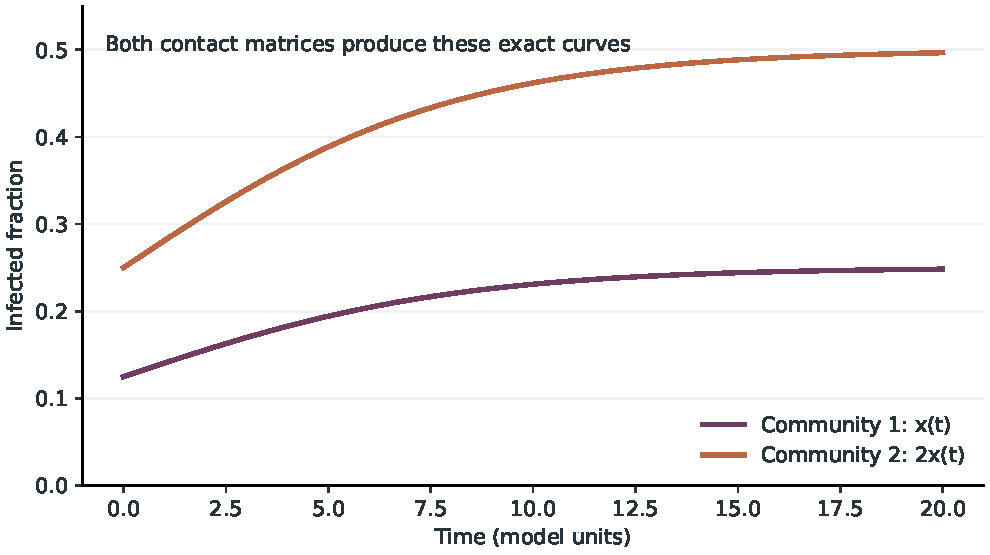
\includegraphics[width=.85\linewidth]{figures/sis_identical_trajectories.pdf}
 \caption{Two distinct contact matrices, given in \eqref{eq:two-community-pair}, produce precisely the same nonstationary infection curves. The different initial fractions and recovery rates rule out block regularity. The curves are the analytic solution \eqref{eq:ray-solution}, evaluated for plotting; their equality follows from the exact matrix identity.}
 \label{fig:identical}
\end{figure}

The case $n=2$ is minimal: in one community, a positive trajectory immediately identifies the single contact weight from \eqref{eq:sis}. Under the source's strictly positive contact-weight assumption, homogeneous recovery and a nonstationary two-community rank defect would force a ray with $\beta>0$. Equation~\eqref{eq:ray-classification} would then force its two coordinates and weighted degrees to agree. The three-community construction above therefore also gives the minimal nonstationary homogeneous-recovery example.

The general invariant-subspace analysis in \cite{PDM2021} assumes that the recovery diagonal matrix separately preserves the proposed subspace. The heterogeneous rays in \eqref{eq:ray-family} do not satisfy that assumption when the $c_i$ differ. Their infection and recovery contributions jointly preserve the ray. This distinction explains why one should not apply a subspace theorem outside its stated hypotheses.

\section{Scope, verification and interpretation}
\label{sec:discussion}

The results concern three different objects: the contact matrix, the observed trajectory, and a continuation error norm. An exact ambiguity in the matrix can coexist with an exactly determined trajectory. Conversely, a uniquely reconstructible matrix can have a poorly conditioned continuation estimate. The examples prove both statements inside positive, bounded parameter classes.

The fixed-dimensional proof does not require a lower bound on any nonzero eigenvalue of the Gram matrix. Its polynomial identity remains valid as the matrix loses rank. This is what the direct compactness argument for Gram matrices misses. The proof relies on classical algebraic closure, and the resulting constant may grow very rapidly with dimension.

The dimension-growth example adds a sharper conclusion than failure of a universal constant. Its explicit cancelling direction gives an exponential lower bound on the optimal constant, and every member of the family remains reconstructible. The contact matrices are complete, the population weights are equal, and the coefficients stay bounded. Thus sparse networks, vanishing population weights and exactly duplicated coordinates are unnecessary for this obstruction.

The Hölder result supplies a dimension-free SIS rate of continuity, including for direct trajectory observations, by applying classical bounded analytic continuation \cite{T2020}. It improves the source's purely qualitative SIS guarantee by displaying one admissible exponent and constant. The negative family is needed separately: ill-conditioning in a larger class of analytic functions would not itself prove that the obstruction occurs inside admissible positive SIS models. We do not determine the optimal modulus of continuity. In particular, the present exponential lower bound for a linear residual estimate does not prove that the Hölder exponent is sharp, and it does not establish failure of every possible linear bound for actual trajectory error. Those are distinct questions.

All finite examples can be verified using rational matrices and symbolic identities. Their analytic proofs do not depend on floating-point eigenvalues or a numerical tolerance for rank. For the dimension-growth family, the positive formula \eqref{eq:positive-convolution} is preferable to summing alternating coordinates in ordinary precision. The latter calculation can lose the small signal through cancellation.

One exact check of reconstruction is available directly from the initial derivatives. Let
\[
 Z_{ik}=[t^k]z_i(t),\qquad i,k=0,\ldots,d,
\]
where $[t^k]$ denotes the ordinary Taylor coefficient for the family \eqref{eq:negative-family}. For each $k$, this coefficient is a polynomial in $\gamma_i$ of degree $k$, with leading term $\tfrac12(-\gamma_i)^k/k!$. This follows inductively from $z_i'=a-(a+\gamma_i)z_i$: the common forcing and multiplication by $a$ contribute only lower powers of $\gamma_i$. The Vandermonde determinant therefore gives
\begin{equation}
 \det Z=
 2^{-(d+1)}(-1)^{d(d+1)/2}
 d^{-d(d+1)/2}\ne0.
 \label{eq:jet-determinant}
\end{equation}
Here $\prod_{0\leq i<j\leq d}(j-i)=\prod_{k=1}^d k!$ cancels the Taylor-factorial denominator. Equation~\eqref{eq:jet-determinant} is an exact arithmetic sanity check on the Volterra reconstruction proof.

The literature boundary should also remain visible. The version of record of \cite{KH2026}, published on 2 May 2026, contains the conjectures addressed here. The prior-art comparison identifies exact antecedents for the polynomial closure method \cite{NY1999}, the homogeneous complete-network solution \cite{PDM2021}, and the general bounded analytic continuation principle \cite{T2020}. A bounded search conducted on 20 October 2026 did not locate the split conclusion for Conjecture 3.11, the quantitative family \eqref{eq:negative-family}--\eqref{eq:exponential-bound}, or the explicit SIS Hölder estimates in the inspected sources. This is a statement about the recorded search, not proof of historical priority. The accompanying evidence record separates these contribution units and records the searches and source comparisons.

\section*{Declarations and availability}

\textbf{Scholarly creator.} Anonymous.

\textbf{Author contributions and AI assistance.} The anonymous scholarly
creator is responsible for the mathematical analysis, software and manuscript.
AI systems assisted with drafting, symbolic checking, adversarial review and
publication preparation. These internal checks are not external peer review
or proof-assistant formalisation.

\textbf{Code and evidence availability.} The public release accompanying this
paper contains the claim--proof map, exact finite checker, hostile semantic
negative control, frozen outputs, figures, hashes and portable replay
instructions. The finite checker tests rational examples and jets through the
reported dimensions; the fixed-dimensional closure and H\"older theorems rest
on the written proofs.

\textbf{Ethics, funding and competing interests.} No human participants,
animals, clinical records or personal data are involved. No external funding
or competing interests are declared.

\begin{thebibliography}{9}
\bibitem{KH2026}
D. Keliger and I. Horv\'ath (2026).
Why is it easier to predict the epidemic curve than to reconstruct the underlying contact network?
\emph{Journal of Mathematical Biology}, \textbf{92}, Article 82.
\url{https://doi.org/10.1007/s00285-026-02401-6}.

\bibitem{NY1999}
D. Novikov and S. Yakovenko (1999).
Trajectories of polynomial vector fields and ascending chains of polynomial ideals.
\emph{Annales de l'Institut Fourier}, \textbf{49}(2), 563--609.
\url{https://doi.org/10.5802/aif.1683}.

\bibitem{PDM2021}
B. Prasse, K. Devriendt and P. Van Mieghem (2021).
Clustering for epidemics on networks: A geometric approach.
\emph{Chaos}, \textbf{31}(6), 063115.
\url{https://doi.org/10.1063/5.0048779}.

\bibitem{KO2013}
Y. Kawano and T. Ohtsuka (2013).
Observability at an initial state for polynomial systems.
\emph{Automatica}, \textbf{49}(5), 1126--1136.
\url{https://doi.org/10.1016/j.automatica.2013.01.020}.

\bibitem{T2020}
L. N. Trefethen (2020).
Quantifying the ill-conditioning of analytic continuation.
\emph{BIT Numerical Mathematics}, \textbf{60}, 901--915.
\url{https://doi.org/10.1007/s10543-020-00802-7}.
\end{thebibliography}
\end{document}
